\documentclass{easychair}

% \usepackage{doc}
\usepackage{setspace}
\usepackage{verbatim}
\usepackage{amssymb}
\usepackage[straightquotes]{newtxtt}

%----Suppress extra space in texttt mode
\AddToHook{cmd/ttfamily/after}{\frenchspacing}

%----Making things more compact
\newcommand{\smalltt}[1]{\small \texttt{#1}}
\newenvironment{packed_itemize}{
\vspace*{-0.3em}
\begin{itemize}
\setlength{\partopsep}{0pt}
\setlength{\itemsep}{1pt}
\setlength{\parskip}{0pt}
\setlength{\parsep}{0pt}
}{\end{itemize}}
\newenvironment{packed_enumerate}{
\vspace*{-0.3em}
\begin{enumerate}
\setlength{\partopsep}{0pt}
\setlength{\itemsep}{1pt}
\setlength{\parskip}{0pt}
\setlength{\parsep}{0pt}
}{\end{enumerate}}
% \renewcommand{\textfraction}{0.07}
% \renewcommand{\topfraction}{0.9}
% \renewcommand{\bottomfraction}{0.9}
% \renewcommand{\floatpagefraction}{0.66}
% \setlength{\floatsep}{2.0pt plus 2.0pt minus 2.0pt}
% \setlength{\textfloatsep}{5.0pt plus 2.0pt minus 0.0pt}

\newcommand{\alex}[1]{{\color{red}{{#1}}}}

\title{Towards StarExec on the AWS Cloud}

\author{
  David Fuenmayor\inst{1}
\and
  Jack McKeown\inst{2}
\and
  Geoff Sutcliffe\inst{2}
}

\institute{
  University of Bamberg,
  Bamberg, Germany\\
  \email{david.fuenmayor@uni-bamberg.de}
\and
  University of Miami,
  Miami, USA\\
  \email{jam771@miami.edu,geoff@cs.miami.edu}
}

\authorrunning{Fuenmayor, McKeown, Sutcliffe}
\titlerunning{Stars in the Clouds}

\begin{document}
\maketitle

%--------------------------------------------------------------------------------------------------
\begin{abstract}
\end{abstract}
%--------------------------------------------------------------------------------------------------
% Geoff
\section{Introduction}
\label{Introduction}

Automated Theorem Proving (ATP) is concerned with the development and use of tools that automate 
sound reasoning: the derivation of conclusions that follow inevitably from facts.
Automated Theorem Proving (ATP) is at the heart of many computational tasks, in particular for
verification \cite{Har06,HH19} and security \cite{Coo18}.\footnote{%
In AWS -
\href{https://aws.amazon.com/what-is/automated-reasoning/}{aws.amazon.com/what-is/automated-reasoning/}, 
\href{https://aws.amazon.com/security/provable-security//}{aws.amazon.com/security/provable-security/}.} 
New and emerging application areas include
chemistry \cite{Yad17}, 
biology \cite{CC+13}, 
medicine \cite{HLB05},
elections \cite{Nip09,BDS17}, 
auctions \cite{CK+15}, 
privacy \cite{Lib20},
law \cite{PS15}, 
ethics \cite{DF+16}, 
religion \cite{OZ11,BW14-ECAI,Hor19},
and business \cite{Han98}.
ATP systems are also used as components of more complex Artificial Intelligence (AI) systems,
and the impact of ATP is thus extended into many facets of society.
% in areas such as 
% knowledge representation \cite{TR+04}, 
% natural language processing \cite{BM05}, 
% planning \cite{NV07}, 
% agents \cite{TBP03}, 
% commonsense reasoning \cite{MS05}, 
% and the semantic web \cite{McG04}.

The Thousands of Problems for Theorem Provers (TPTP) World \cite{Sut17} is a well established 
infrastructure that supports research, development, and deployment of ATP systems.
The TPTP World includes 
the TPTP problem library \cite{Sut17},
the TSTP solution library \cite{Sut10},
standards for writing ATP problems and reporting ATP solutions \cite{SS+06,Sut08-KEAPPA},
tools and services for processing ATP problems and solutions \cite{Sut10},
and it supports the the annual CADE ATP System Competition (CASC) \cite{Sut16}.
Since its first release in 1993 the ATP community has used the TPTP World as an appropriate and 
convenient infrastructure for ATP system development, evaluation, and application.
The TPTP World has a diverse, engaged, and sustained user community, with various parts of the 
TPTP World being deployed in a range of applications in both academia and industry.\footnote{%
TPTP has contributed to recognized research in 627 publications that cite \cite{Sut17},
according to Google Scholar.}
The web page \href{https://www.tptp.org}{\tt www.tptp.org} provides access to all components.

The TPTP problem library was motivated (see Section~\ref{TPTP}) by the need to provide support
for meaningful ATP system evaluation.
This need was also (or became) evident in other logic solver communities, e.g., 
SAT~\cite{HS00-SATLIB} and SMT~\cite{BST10}.
For many years testing of logic solvers was done on individual developer's computers. 
In 2010 a proposal for centralised hardware and software support was developed,
and in 2011 a \$2.11 million NSF grant\footnote{%
NSF Awards 1058748 and 1058925, led by Aaron Stump and Cesare Tinelli at the University of Iowa} 
was obtained.
This grant led to the development and availability of StarExec Iowa~\cite{SST14} in 2012,
and a subsequent \$1.00 million grant\footnote{%
NSF Award 1730419} in 2017 expanded StarExec to Miami.
StarExec has been central to much progress in logic solvers over the last 10 years, supporting
16 logic solver communities, used for running many annual competitions~\cite{BB+19}, and 
supporting many many users.
StarExec Iowa provides community infrastructure for many logic solver communities,
e.g., ASP, QBF, SAT, SMT, Termination, etc, while
StarExec Miami is used by the ATP community.
StarExec Miami has features that take advantage of TPTP standards, and is also used to host CASC.

It was recently announced that StarExec Iowa will be decommissioned. 
The maintainer of StarExec Iowa explained that ``the plan is to operate StarExec as usual for 
competitions Summer 2024 and Summer 2025, and then put the system into a read-only mode for one 
year (Summer 2025 to Summer 2026)''.
The current static StarExec Miami service was funded by a 3-year NSF grant in 2017, which paid 
for the hardware and three years of system administration.
The hardware is still hosted by the University of Miami High Performance Computing group,
funded on a shoe-string budget by the TPTP World.
While StarExec Miami will continue to operate while funding is available, but it will not be able
to support the large number of logic solver communities that use the larger StarExec Iowa cluster.
In the long term StarExec will necessarily have to migrate to a commonly available compute service.
This project will convert the current static StarExec service into a flexible Kubernetes-based 
service that runs in AWS.

\paragraph{This paper is organized as follows:}

%--------------------------------------------------------------------------------------------------
% David
\section{Background}
\label{Background}

Containerization

Kubernetes

%--------------------------------------------------------------------------------------------------
% Jack and Geoff and David
\section{Containerizing ATP Systems}
\label{ATPSystems}

%--------------------------------------------------------------------------------------------------
% Geoff and Divid
\section{Into the AWS Cloud}
\label{AWSCloud}

Figure~\ref{AWSArchitecture} shows the architecture of the final implemented system.

\begin{figure}[htb]
\begin{center}
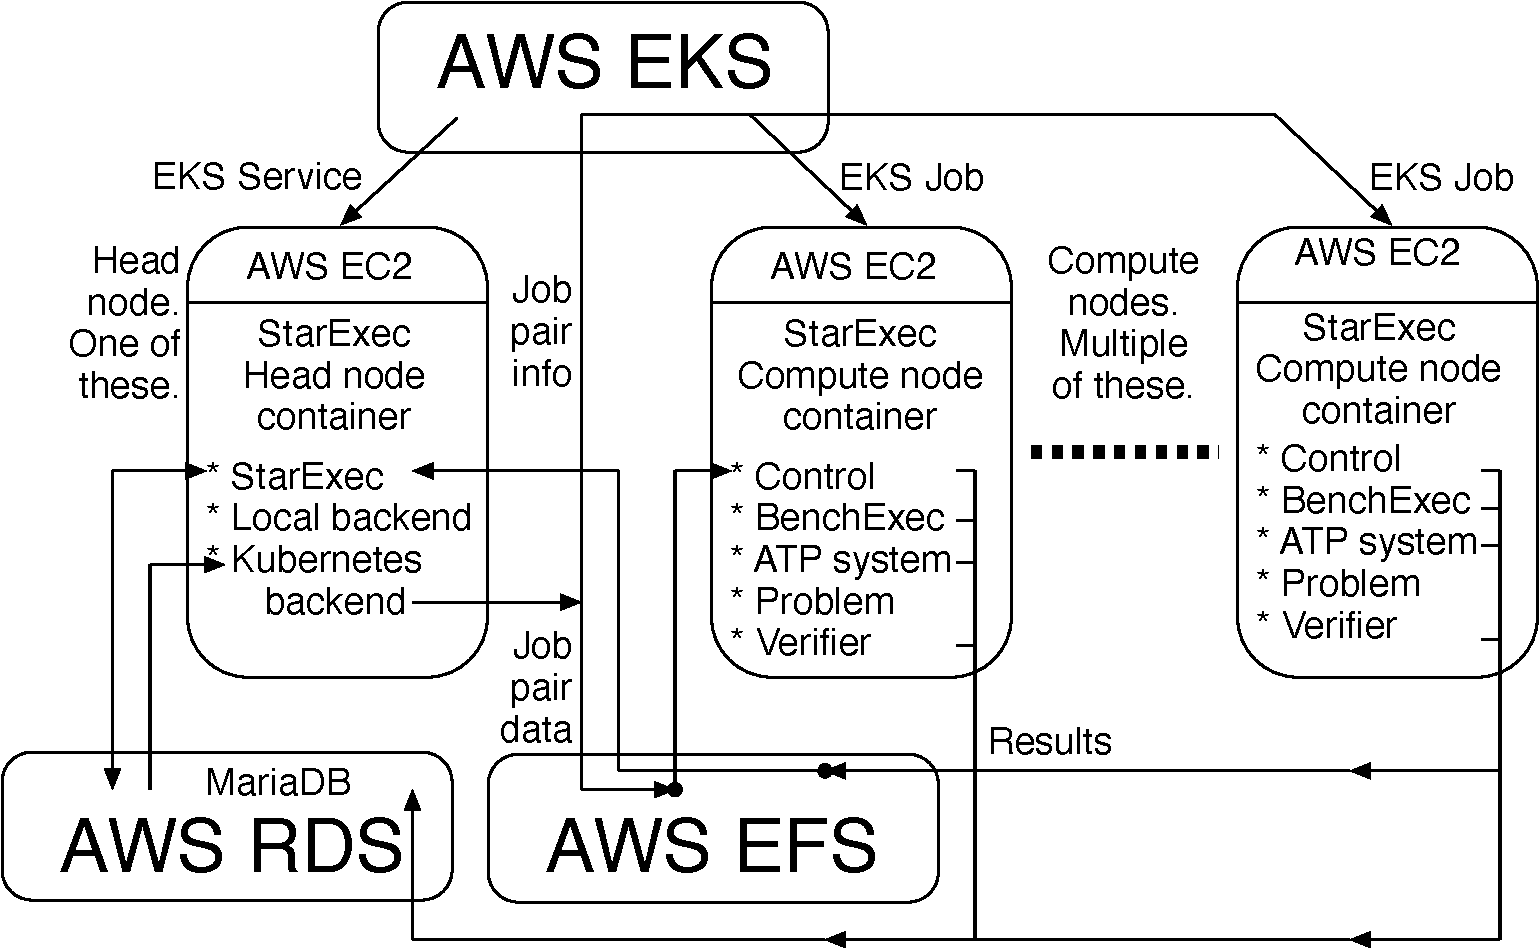
\includegraphics[width=0.8\textwidth]{AWSArchitecture}
\caption{AWS architecture}
\label{AWSArchitecture}
\end{center}
\end{figure}

%--------------------------------------------------------------------------------------------------
% Geoff
\section{Conclusion}
\label{Conclusion}

This paper 
%--------------------------------------------------------------------------------------------------
\bibliographystyle{plain}
\bibliography{Bibliography.bib}
%--------------------------------------------------------------------------------------------------
\end{document}
%--------------------------------------------------------------------------------------------------
